\section{L-systémy}\label{sec:L-systemy}

Uvedeme tuto kapitolu s~ohledem na předchozí obsah trochu netradičně a od matematiky se (alespoň zdánlivě) na chvíli odkloníme. Podíváme se na fraktály,~s jejichž způsobem popisu přišel roku 1968 maďarský biolog \name{Aristid Lindenmayer} (1925--1989) a který (možná pro někoho i~překvapivě) má základy především v~informatice. \citep[str. 2]{Prusinkiewicz1990}

K popisu specifického druhu fraktálů lze využít znalosti z \emph{teorie formálních jazyků} a \emph{teorie automatů}, na jejímž počátku stál (mj.) britský matematik a informatik \name{Alan Turing} (1912--1954). Ten ve svém článku \emph{On Computable Numbers, with an Application to the Entscheidungsproblem} z roku 1936 zavedl koncept abstraktního stroje dnes známého jako \emph{Turingův stroj}\index{Turingův stroj}, jednoduché zařízení s výpočetními schopnostmi již tehdy porovnatelnými se současnými počítači. Jeho princip fungování přitom není nikterak složitý. Pomineme-li nyní matematickou definici Turingova stroje, lze říci, že sestává ze tří hlavních částí:
\begin{enumerate}
    \item \textbf{Oboustranně nekončná páska.} Páska je rozdělena na políčka, z nichž každé může obsahovat některý symbol z z předem známé abecedy (formálně vzato množiny) znaků.
    \item \textbf{Čtecí/zapisovací hlava.} Hlavu si můžeme představit jako čtecí/zapisovací "okénko", které stojí právě nad jedním políčkem pásky. V každém kroku stroj:
    \begin{itemize}
        \item přečte symbol pod hlavou,
        \item podle svého stavu a právě přečteného symbolu rozhodne, jakou akci provést.
    \end{itemize}
    \item \textbf{Řídicí jednotka.} Řídí chování stroje pomocí konečné množiny stavů
    \[Q=\set{q_0,q_1,\ldots,q_n}.\]
    Přechodová funkce $\delta$ pro (ne nutně všechny) dvojice $(\text{stav},\text{znak})$ udává:
    \begin{itemize}
        \item jaký symbol má hlava na pásku zapsat (může přepsat stávající symbol nebo nechat stejný),
        \item do jakého stavu se stroj přepne,
        \item jak se posune hlava: doleva (L), doprava (R) nebo zůstane (N).
    \end{itemize}    
\end{enumerate}
Výpočet pak probíhá takto:
\begin{enumerate}
    \item Stroj začíná ve stavu, který je stanovený jako počáteční. Na pásce je vložen vstup (řetězec symbolů), zbytek pásky je prázdný.
    \item Vždy podle přechodové funkce stroje:
    \begin{itemize}
        \item přečte, co je pod hlavou,
        \item zapíše (případně přepíše) symbol,
        \item přesune hlavu,
        \item přejde do dalšího stavu.
    \end{itemize}
    \item Pokud stroj nemá definovaný přechod pro aktuální stav a symbol na pásce, zastaví se. Pokud stroj skončil ve stavu, který je označený jako přijímající, pak stroj slovo \textbf{přijal}, jinak jej \textbf{odmítá}.
\end{enumerate}
\begin{figure}[h]
    \centering
    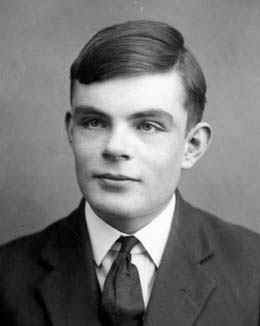
\includegraphics[width=.4\textwidth]{Alan-Turing.jpeg}
    \caption[Alan Turing,~1871--1956]{Alan Turing\footnote{Převzato z~\cite{OConnorTuring2025}},~1912--1954}
    \label{fig:alan-turing}
\end{figure}
V té době se zabýval otázkou, kterou v roce 1928 položil známý německý matematik \name{David Hilbert} (1862--1943), jež je známá pod názvem \emph{"Entscheidungsproblem"}\index{Entscheidungsproblem}\footnote{Anglicky \emph{The Decision problem}\index{The Decision problem}, česky přeložitelné jako \emph{"rozhodovací problém"}. Zde však poznamenejme, že onem český termín se používá i v související teorii složitosti a vyčíslitelnosti, má však podstatně jiný význam.}. Problémem bylo, zda existuje algoritmus, který o každém tvrzení je schopný rozhodnout (v konečném čase), zda je či není pravdivé. Později Alan Turing tento problém přeformuloval takto: \emph{Existuje program, který o jiném programu na vstupu rozhodne, zda se zastaví, či nikoliv?} David Hilbert byl ve svých vizích optimistický, avšak nakonec Alan Turing dokázal, že \textbf{takový algoritmus nemůže existovat}. Způsob, jakým Turing došel onomu výsledku, byl v konečném důsledku vlastně až překvapivě jednoduchý a existuje pro něj velké množství popularizačních materiálů\footnote{Pokud by se chtěl čtenář dozvědět více o této problematice a teorii s ní související, doporučuji např. knihu \cite{Motwani2003}}.
\begin{figure}[h]
    \centering
    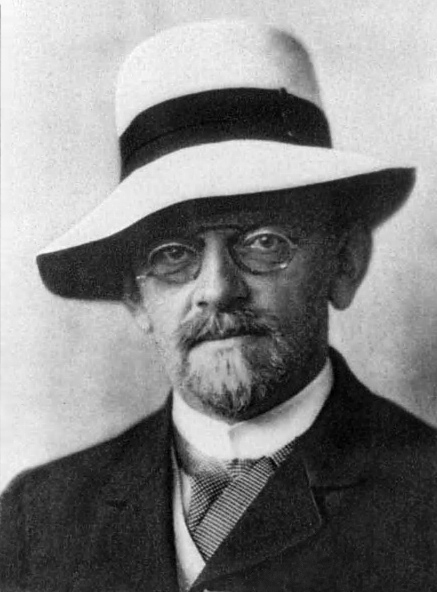
\includegraphics[width=.4\textwidth]{David-Hilbert.jpg}
    \caption[David Hilbert,~1862--1943]{David Hilbert\footnote{Převzato z~\cite{OConnorHilbert2025}},~1862--1943}
    \label{fig:david-hilbert}
\end{figure}
Alan Turing dal základ dnešní teoretické informatice. Turingův stroj, co by výpočetní model, stojí na samotném vrchlu hierarchie dalších výpočetních modelů\footnote{Mezi ně patří jmenovitě tzv. \textit{lineárně omezený automat}\index{automat!lineárně omezený}, \emph{zásobníkový automat}\index{automat!zásobníkový}, \emph{deterministický}\index{automat!deterministický} a \emph{nedeterministický konečný automat}\index{automat!nedeterministický}.}, které jsou však svoji výpočetní silou slabší.  Později pak americký matematik \name{Noam Chomsky} (1928--současnost) popsal celkem 4 základní třídy tzv. \emph{formálních jazyků}, které jsou dnes souhrně známé pod názvem \emph{Chomského hierarchie}\index{Chomského hierarchie}. Za formální jazyk považujeme určitou množinu slov (rětězců). Chomského hierarchie zařazuje každý jazyk do jedné ze tříd podle výočetního modelu, který jej přijímá, resp. typu tzv. \emph{formální gramatiky}, která slova z něj generuje. O gramatikách a obecně určitém základu teorie formálních jazyků si ještě budeme podrobněji povídat později. O hlubší související teorii se čtenář může více dozvědět např. v knize \cite{Motwani2003}.

\subsection{Odbočka k formálním jazykům a gramatikám}\label{subsec:formalni-jazyky-a-gramatiky}

V úvodu této sekce jsme si již trochu přiblížili historické pozadí teorie formálních jazyků a automatů (tou se již dále zabývat nebudeme, nicméně bylo by při nejmenším neslušné ji zde alespoň nezmínit vzhledem k její přímé souvislosti). Ačkoliv tento text si neklade za cíl seznámit čtenáře se všemi podrobnostmi, byly zmíněny určité termíny, jejichž význam bude dobré si objasnit, konkrétně
\begin{itemize}
    \item \emph{formální jazyk}\index{formální!jazyk}
    \item a \emph{formální gramatika}.\index{formální!gramatika}
\end{itemize}
